\documentclass[11pt,a4paper]{article}
\usepackage[english]{babel}
\usepackage[T1]{fontenc}
\usepackage{lmodern,microtype}
\usepackage[margin=2cm,top=1.8cm]{geometry}
\usepackage{titlesec}\titlespacing*{\section}{0pt}{1.1em}{0.4em}
\usepackage{amsmath,amssymb}\usepackage{eurosym}
\usepackage{booktabs,tabularx,array}
\usepackage{graphicx,float}\usepackage[font=small,labelfont=bf]{caption}
\usepackage{enumitem}\setlist{nosep,leftmargin=1.4em}
\usepackage[dvipsnames]{xcolor}
\usepackage[colorlinks=true,urlcolor=NavyBlue,linkcolor=NavyBlue]{hyperref}
\setlength{\parskip}{0.45em}\setlength{\parindent}{0pt}
\newcommand{\scoreFinal}{18.30}
\newcommand{\scoreStrict}{18.20}
\newcommand{\coFinal}{17.25}
\newcommand{\costFinal}{20.75}
\newcommand{\timeFinal}{13.9}
\newcommand{\timeExtrap}{16}
\newcommand{\zipKB}{194}
\newcommand{\cyclesDay}{1.12}
\newcommand{\exported}{11038}
\newcommand{\configFinal}{$H=24$ h, $V=1.11\,\bar\lambda$, $z=0.42$, $\varepsilon=0.018$}
\newcommand{\calibTable}{0.0 & 1.0 & 0.02 & yes & 20.01 & 18.01\\
0.0 & 1.0 & 0.06 & yes & 19.92 & 17.96\\
0.5 & 1.0 & 0.02 & yes & 20.22 & 18.30\\
0.5 & 1.0 & 0.06 & yes & 20.11 & 18.21\\
1.0 & 1.0 & 0.02 & yes & 20.05 & 18.14\\
1.0 & 1.0 & 0.06 & yes & 19.94 & 18.04\\
0.5 & 0.6 & 0.02 & yes & 20.21 & 18.29\\
0.5 & 1.0 & 0.02 & no & 17.44 & 15.91\\
}
\newcommand{\scoreRidge}{16.74}
\newcommand{\scoreNoPred}{15.91}
\newcommand{\scoreLamPerf}{18.94}
\newcommand{\scoreNPerf}{19.01}
\newcommand{\scoreAllPerf}{19.70}
\newcommand{\scoreOracle}{19.92}
\newcommand{\scoreOracleStd}{7.61}

\newcommand{\optResults}{\begin{table}[H]\centering\small
\begin{tabular}{lccccccccc}\toprule
 & $z$ & $V/\bar\lambda$ & $\varepsilon$ & $\alpha_D$ & $\alpha_S$ & $\alpha_\lambda$ & $s_S$ & $s_\lambda$ & \textbf{Real score}\\\midrule
starting point & 0.50 & 1.00 & 0.020 & 1.00 & 0.00 & 0.00 & 1.00 & 1.00 & 18.26\\
\textbf{potential optimum} & 0.42 & 1.11 & 0.018 & 1.00 & 0.00 & 0.04 & 0.96 & 0.93 & 18.30\\
perfect information (control) & 0.61 & 0.78 & 0.016 & 0.85 & 0.00 & 0.00 & 0.95 & 0.73 & 19.67\\
\bottomrule\end{tabular}
\caption{Coefficients before and after optimising the potential (23 local Nelder--Mead runs in 4 workers;
688 scenario-set evaluations). ``Real score'': the 12 concatenated pseudo-test weeks. The last row is the
perfect-information case: the ceiling of the controller, with the global oracle at 19.92.}
\end{table}
\begin{figure}[H]\centering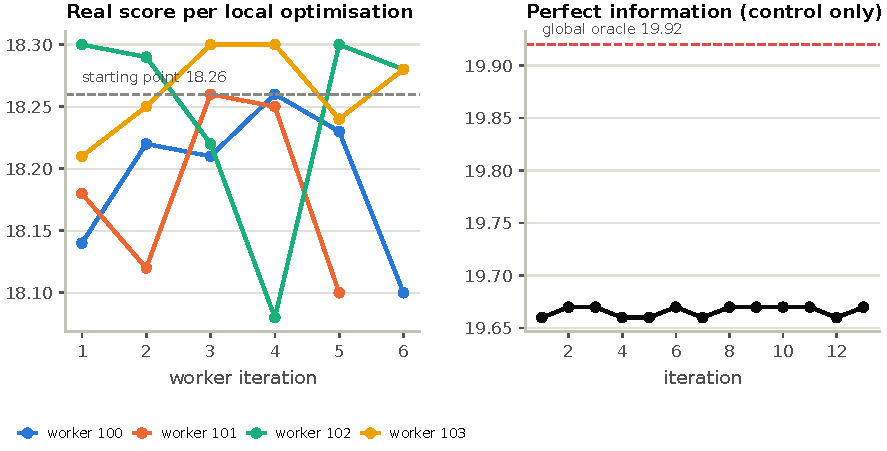
\includegraphics[width=\linewidth]{fig/potential.pdf}
\caption{Left: real score reached by each worker after each local optimisation (the shared record only goes up). Right: the perfect-information worker.}\end{figure}
}


\begin{document}
\begin{center}
{\LARGE\bfseries Forecasting + linear programming for the campus battery}\\[4pt]
{\large Datathon FME 2026 --- AED $\times$ UPC Sostenible battery challenge}\\[3pt]
{\small Team EngIAnyers \quad·\quad November 2026 \quad·\quad \url{https://github.com/Anty48/Datathon2026}}
\end{center}

\section*{Summary}
\begin{itemize}
  \item \textbf{Task.} Write a \texttt{BatteryAgent} that, every hour, chooses the charge/discharge set point $u_t$ of the campus battery so as to cut the CO$_2$ emissions (weight 0.7) and the electricity bill (weight 0.3) of the campus with respect to having no battery, with a penalty for every physically impossible request.
  \item \textbf{Physics first.} The score is \emph{linear} in the energy imported from the grid, so the whole problem collapses into minimising $\sum_t\lambda_t g_t$ with a single \textbf{effective price} $\lambda_t=c_t+\kappa\pi_t$ (CO$_2$ intensity plus $\kappa$ times the price). With $\lambda$ known, the optimal schedule is a small linear program (LP) solved every hour on a receding horizon.
  \item \textbf{Standard mode} (2\,MWh, 24\,h of perfect market forecast): the LP agent scored \textbf{6.43 on the public leaderboard}, which is the plateau every strong team hits (6.44): it is the physical ceiling of the problem. Our local perfect-information oracle confirms it (5.58 vs.\ 5.52 for the agent on our pseudo-test).
  \item \textbf{Hard mode} (6\,MWh, $\pm$1500\,kW, solar $\times$12, only \textbf{3\,h} of market forecast): now one has to \emph{forecast} the effective price, the demand and the solar for the rest of the day. Agent v3 combines ridge regressions and \textbf{forecasting by analogy} (kernel-weighted average of the most similar historical days) with an LP that has an explicit grid-import variable and a \textbf{safety margin} on discharge. Leaderboard: 20.24 with ridge forecasts, \textbf{21.78} with analogs. Locally (1725\,h of pseudo-test): \textbf{\scoreFinal{}} points (\coFinal\,\% CO$_2$, \costFinal\,\% cost), \scoreStrict{} in strict mode, zero violations, \timeFinal\,s, against \scoreOracle{} for an oracle that knows the future.
\end{itemize}

\begin{figure}[H]\centering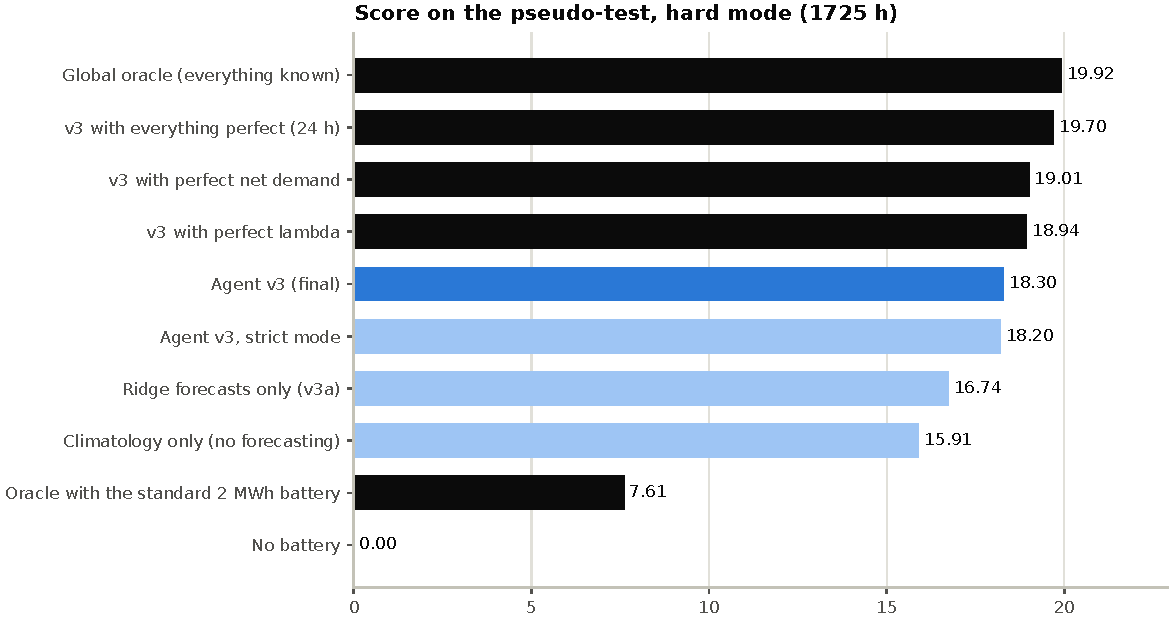
\includegraphics[width=\linewidth]{fig/comparison.pdf}
\caption{Score on the local pseudo-test, hard mode. Black: bounds that use information the agent does not have. Dark blue: final agent.}\end{figure}

\section*{1. The physics of the problem}
\textbf{Dynamics.} With set point $u_t$ (kW, $>0$ charge, $<0$ discharge, 1\,h steps) and round-trip efficiency 90\,\% split evenly, $\eta=\sqrt{0.9}$,
\[
E_{t+1}=E_t+\eta\,u_t^+-\frac{u_t^-}{\eta},\qquad 0\le E_t\le E_{\max},\qquad |u_t|\le P .
\]
The campus draws $D_t-S_t+u_t$ from the grid (demand minus solar plus battery). Exported energy is worth nothing (0\,\euro, no CO$_2$ credit), so the grid import is $g_t=\max(D_t-S_t+u_t,0)$.

\textbf{Score.} $\text{Score}=\max\big(0,\,0.7\,\Delta\text{CO}_2\%+0.3\,\Delta\text{Cost}\%-0.2\,N_{\text{viol}}\big)$, with $\Delta X\%=100\,(X_0-X)/X_0$ relative to the campus without battery. Since $X_0$ is a constant, the score is a linear functional of the import vector $g$:
\[
\text{Score}\propto-\sum_t\Big(\tfrac{0.7}{\text{CO}_2^{(0)}}\,c_t+\tfrac{0.3}{\text{Cost}^{(0)}}\,\pi_t\Big)g_t\ \propto\ -\sum_t\lambda_t\,g_t,\qquad
\lambda_t=c_t+\kappa\,\pi_t,\quad \kappa=\frac{0.3}{0.7}\,\frac{\text{CO}_2^{(0)}}{\text{Cost}^{(0)}} .
\]
$\kappa$ is the exchange rate between euros and kilograms of CO$_2$ that the scoring formula implies: 0.2466\,kg/\euro{} on train, 0.2592 on the public test week (71\,816\,kg / 118\,746\,\euro); we use $\kappa=0.259$. Two consequences guide everything else:
\begin{itemize}
  \item Arbitrage only pays when $\lambda_{\text{high}}/\lambda_{\text{low}}>1/\eta^2=1.11$: every kWh that goes through the battery loses 10\,\%.
  \item Violations are entirely avoidable: the agent clips its own output with the simulator's exact formula ($\eta=\sqrt{0.9}$, not a rounded 0.9487 --- the official template loses 9 violations because of that rounding).
\end{itemize}

\textbf{Local validation.} The hidden test set is the last week of every month. We imitate it with days 15--21 of every month of the training year (12 blocks, 1725\,h, concatenated with time jumps exactly as the server does) and fit every model on the remaining days only (the one exception, the final choice of eight control coefficients, is discussed in Section~6). A \emph{strict} mode additionally truncates the market forecast at the end of each block, in case the server does so.

\section*{2. Standard mode: the LP is already optimal}
Every hour the standard agent solves
\[
\min_{u^\pm\ge0}\ \sum_{k=0}^{H-1}\lambda_k\,(u_k^+-u_k^-)-V E_H\quad\text{s.t.}\quad 0\le E_k\le 2000,\ u^+_k\le 500,\ u^-_k\le \bar N_k ,
\]
over the 24 known hours plus 12 climatological ones, with the climatological net demand $\bar N$ (hour $\times$ weekday $\times$ month) as an upper bound on discharge and a terminal value $V$ for the energy left at the end. The bound never binds (the campus net demand is always far above 500\,kW), so the only thing that matters is $\lambda$, which is given. Our global LP with perfect information scores 5.58 on the pseudo-test and the agent 5.52; the receding horizon costs nothing. On the leaderboard this agent scored \textbf{6.43}, i.e.\ the 6.44 plateau: a physical ceiling, not a modelling one.

\section*{3. Hard mode: what changes}
\begin{tabularx}{\linewidth}{@{}lXX@{}}
\toprule
 & \textbf{Standard} & \textbf{Hard}\\
\midrule
Battery & 2000 kWh, $\pm$500 kW & 6000 kWh, $\pm$1500 kW (read from \texttt{obs}) \\
Solar & peak 144 kW; never exceeds demand & $\times$12: peak 1730 kW; surplus in 9\,\% of the hours (up to 1100 kW)\\
Market forecast & 24 h of $\pi$ and $c$ (perfect) & 3 h; the rest must be forecast\\
Telemetry & last hour's consumption and solar & + irradiance, temperatures and wind\\
Consequence & discharge bound never binds; 24 h is enough & the future net demand $N=D-S$ decides how much to discharge; the future $\lambda$ decides when\\
\bottomrule
\end{tabularx}

The battery now moves about 20\,\% of the campus energy, and solar surpluses are \emph{free} energy (0\,\euro, 0\,kg), so scores jump from $\sim$6 to $\sim$20. With the standard battery and solar $\times$12 the oracle would reach only \scoreOracleStd{}: the size of the battery is what opens the margin. Discharging 1500\,kW blindly, however, exports energy at 0 whenever the demand turns out lower than expected: the agent must forecast.

\section*{4. Forecasting}
\textbf{Ridge regressions.} For every horizon $k=0,\dots,23$ a linear model, fitted by regularised least squares on train, uses only quantities the agent can compute in real time:
\begin{align*}
\hat\lambda_{t+k} &= w_0 + w_1\,\bar\lambda(h,\text{weekend},\text{month}) + w_2\,a_{t+k-24} + w_3\,a_{t+k-48} + w_4\,a_{t+2} + w_5\,a_{t} + w_6\,\bar a_{24\,\mathrm h},\\
\hat D_{t+k} &= w_0 + w_1\,\bar D(h,\text{dow},\text{month}) + w_2\,(D_{t-1}-\bar D_{t-1}) + w_3\,(D_{t+k-24}-\bar D_{t+k-24}),\\
\hat S_{t+k} &= w_0 + w_1\,\bar S + w_2\,\bar S\,k^{\text{recent}} + w_3\,\bar S\,k^{\text{yesterday}},
\end{align*}
where bars are climatologies, $a=\lambda-\bar\lambda$ is the anomaly, $\bar a_{24\mathrm h}$ the mean anomaly of the last 24 known hours and $k$ the clearness index (measured over climatological solar). These are the adaptation mechanisms an ``odd'' day calls for: if prices are high today, if the campus consumes more than usual or if it is cloudy, the anomalies propagate to the rest of the day with weights that decay with $k$ (fitted, not imposed). Each model also stores the standard deviation $\sigma_k$ of its error, used by the controller as a safety margin.
\begin{figure}[H]\centering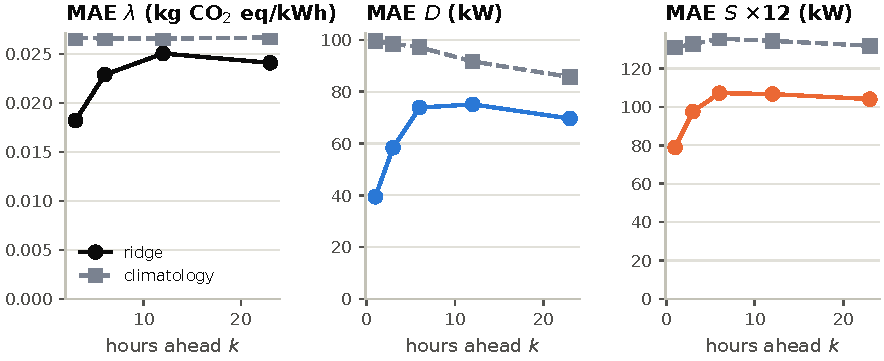
\includegraphics[width=\linewidth]{fig/predictors.pdf}
\caption{Mean absolute error of the ridge forecasts on the pseudo-test vs.\ horizon. Forecasting $\pi$ and $c$ separately and recombining them was worse than forecasting $\lambda$ directly.}\end{figure}

\textbf{Forecasting by analogy (``which past days does today look like?'').} For $\lambda$ and $S$ the linear model flattens the peaks. The alternative imposes no shape at all: the forecast is the \textbf{average of what happened after the most similar historical hours}, weighted by similarity (Nadaraya--Watson kernel regression),
\[
\hat y_{t+k}=\frac{\sum_i w_i\,y_{i+k}}{\sum_i w_i},\qquad w_i=\exp\Big(-\tfrac12\sum_j \frac{(f_j-f_{ij})^2}{h_j^2}\Big),
\]
comparing only hours with the same hour of day. The features $f_j$ are the observable state: last hour's irradiance, ambient and panel temperature, consumption and solar (and its clearness index), the three known $\lambda$ anomalies, their 24\,h level, the month (sine and cosine) and the day type. The bandwidths $h_j$ are the coefficients of the model, fitted on train by coordinate descent on the forecast error with the $\pm$3 days around each query left out ($h_j=\infty$ switches a feature off; the wind sensor is constant in the data and is not used). An instructive detail: finer bandwidths slightly \emph{worsen} the mean error of $\lambda$ (0.0168 $\to$ 0.0179) but \emph{raise} the score (18.15 $\to$ 18.26), because the controller rewards getting the \emph{shape} of the peaks right, not the average. For $\lambda$ the 6\,h-ahead error drops from 0.023 (ridge) to 0.014. The analog table (4205 training hours with their features and the following 24\,h) ships inside the zip (\texttt{analogs.json}, 2.5\,MB) and a query costs under a millisecond.

\section*{5. The controller: LP with explicit import and a safety margin}
\begin{align*}
\min_{u^\pm,g}\ & \sum_{k=0}^{H-1}\big(\hat\lambda_k\,g_k+\varepsilon\bar\lambda\,u^-_k\big)-V\,E_H\\
\text{s.t.}\ & g_k\ge \hat N_k+u^+_k-u^-_k,\quad g_k\ge0,\quad 0\le E_k\le E_{\max},\\
& 0\le u^+_k\le P,\quad 0\le u^-_k\le\min\!\big(P,\max(0,\hat N_k-z\,\sigma_k)\big).
\end{align*}
$g_k$ is the grid import: when $\hat N_k<0$ (surplus) charging up to $-\hat N_k$ is free, and discharging above the demand saves nothing (the LP ``knows'' it because $g$ stays at 0). The margin $z\sigma_k$ is the risk decision: discharge only down to the net demand we are reasonably sure will exist. The small $\varepsilon$ discourages discharges with no benefit, and $V$ values the energy left at the end of the horizon. The Lagrange multipliers of the energy constraints are the \emph{shadow price} of a stored kWh at each hour: the LP charges exactly when $\hat\lambda_k\eta$ is below that shadow price and discharges when $\hat\lambda_k/\eta$ is above it. The blend between ridge and analog forecasts uses weights $\alpha_D,\alpha_S,\alpha_\lambda$ (1 = ridge only) and bandwidth scale factors $s_S,s_\lambda$.

\textbf{Grid sweep on train (val only reports).} With the forecasting blend fixed at its final values:
\begin{table}[H]\centering\small
\begin{tabular}{cccccc}\toprule
$z$ & $V/\bar\lambda$ & $\varepsilon$ & forecasting & \textbf{Score train} & \textbf{Score val}\\\midrule
\calibTable
\bottomrule\end{tabular}
\caption{Without the margin ($z=0$) the agent loses $\sim$0.3 points by exporting on low-demand days; without forecasting it loses much more.}\end{table}

\section*{6. Continuous optimisation of the coefficients: the potential $\Phi(\theta)$}
To keep improving without hand tuning we maximise a \textbf{potential} over the controller and blending coefficients,
\[
\theta=(z,\;V,\;\varepsilon,\;\alpha_D,\;\alpha_S,\;\alpha_\lambda,\;s_S,\;s_\lambda),\qquad
\Phi(\theta)=\frac{1}{|\mathcal S|}\sum_{s\in\mathcal S}\text{Score}_s(\theta),
\]
where $\mathcal S$ is a set of scenarios: real pseudo-test weeks \textbf{plus randomly perturbed weeks} (random demand level, autocorrelated noise and 6--12\,h sensor drop-outs, different cloudiness every day, random price and CO$_2$ levels, weather consistent with the solar). The perturbations force $\theta$ to be good on odd days too, not only on average. The score is a non-differentiable function of $\theta$ (each evaluation is a full simulation), so it is maximised with Nelder--Mead; several workers run in parallel with different seeds and scenario samples (\texttt{src/optimize\_parallel.py}), start from the best known $\theta$ plus a random jump, and share a record that is only overwritten if a candidate improves the score on the 12 real concatenated weeks (the server's criterion). An extra worker gives the agent the real $\lambda$, $D$ and $S$ and optimises only $(z,V,\varepsilon)$: it measures how far the \emph{controller} can go when forecasting is not the limit. The final configuration is \configFinal. Note that, unlike the forecasting models (fitted on train only), these eight coefficients are selected by their score on the pseudo-test weeks, so the local score of the final agent is slightly optimistic; the gain over the hand-tuned agent (18.26) is small and was kept because it also holds on the perturbed scenarios.

\optResults

\section*{7. Results and diagnosis}
\begin{figure}[H]\centering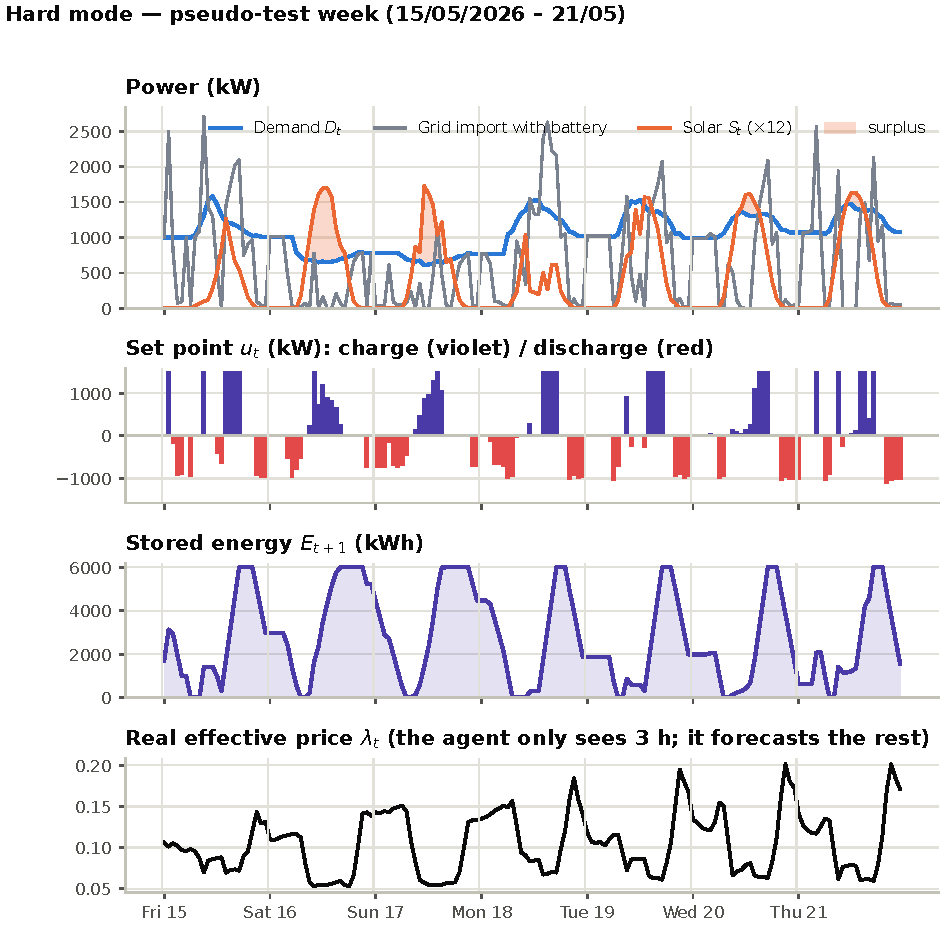
\includegraphics[width=\linewidth]{fig/week.pdf}
\caption{One pseudo-test week. At midday solar exceeds demand (orange area): the battery absorbs the surplus at zero cost and discharges in the evening and at dawn. The grey line (actual import) shows the peaks being shaved. Equivalent cycles: \cyclesDay{} per day; energy exported over the whole pseudo-test: \exported{} kWh.}\end{figure}
\begin{figure}[H]\centering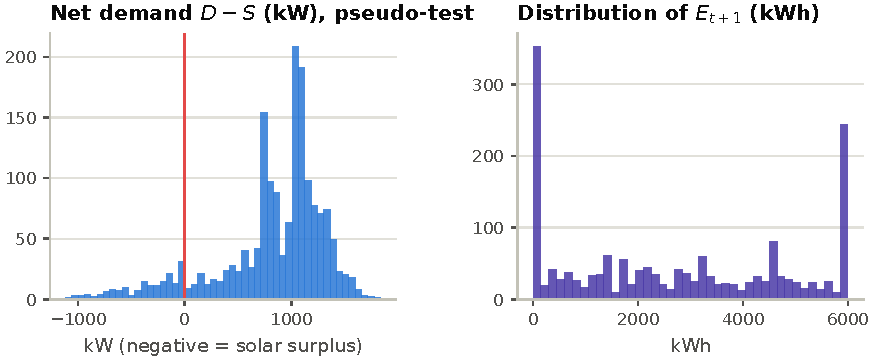
\includegraphics[width=\linewidth]{fig/usage.pdf}
\caption{Left: distribution of the net demand (negative = surplus). Right: the battery sweeps its whole 0--6000\,kWh range.}\end{figure}

\textbf{Where is the gap to the ceiling?} Replacing, inside the agent itself, forecasts by the real values:
\begin{itemize}
  \item climatology only (no forecasting): \scoreNoPred; \quad ridge forecasts: \scoreRidge; \quad \textbf{final agent: \scoreFinal}.
  \item with perfect $\lambda$: \scoreLamPerf; \quad with perfect net demand: \scoreNPerf; \quad with everything perfect over 24\,h: \scoreAllPerf; \quad global oracle: \scoreOracle.
  \item The 24\,h receding horizon costs almost nothing (\scoreAllPerf{} vs.\ \scoreOracle). The remaining gap is split roughly evenly between the effective price and the net demand forecasts. Our own submissions scored 1.19--1.21 times their local values on the server, which puts the server-side oracle around 24: the leaderboard top (23.23) is close to perfect information.
\end{itemize}

\section*{8. Rules, robustness and run time}
\begin{itemize}
  \item Imports: \texttt{json}, \texttt{math}, \texttt{pathlib}, \texttt{typing}, \texttt{numpy}, \texttt{pandas} (Timestamp) and \texttt{scipy.optimize.linprog}. Passes the official \texttt{check\_submission.py}; zip of \zipKB{} KB with \texttt{agent.py}, \texttt{predictors.json} and \texttt{analogs.json} at its root.
  \item Generic: reads \texttt{cap\_max\_kwh} and \texttt{power\_max\_kw} from \texttt{obs} (2000/500 if missing), uses however many market hours are given (3 or 24), and tolerates a missing or textual \texttt{timestamp}, short lists and missing keys; the exact physical clip guarantees zero violations in any mode.
  \item Time: \timeFinal{} s for 1725 h ($\approx$\timeExtrap{} s for the 2016 test hours; limit 60 s), after indexing the history by integer hours (the first version spent twice as long on date arithmetic, not on the LP).
  \item The date jumps between test weeks reset the clearness index and leave the first day of each block without a ``yesterday'': the predictors were fitted including those cases (yesterday's anomaly $=0$).
\end{itemize}

\section*{Appendix: how to reproduce}
Place the organisers' package in \texttt{data/} and \texttt{starter\_kit/} (see the README), then from the repository root:
{\footnotesize\begin{verbatim}
python src/hard_env.py             # hard-mode data (pv x12 + weather) and simulator with a 3 h horizon
python src/predictors.py           # ridge predictors          -> agent/predictors.json
python src/analogs.py              # analog bandwidths         -> agent/analogs.json
python src/oracle.py               # perfect-information ceiling
python src/diagnose.py             # perfect lambda / net demand / everything inside the agent
python src/calibrate.py            # grid sweep of z, V, eps on train
python src/optimize_parallel.py --minutes 40     # potential optimisation (optional, long)
python src/finalize.py --best results/opt/best.json
python src/figures.py && python src/summarize_opt.py && python src/make_viewer.py
cd report && pdflatex report.tex && pdflatex report.tex
\end{verbatim}}
\end{document}
